\setcounter{section}{0}

\section{Lecture 1: Introduction, Degrees of Freedom, and Lagrangian Dynamics}

\subsection{Introduction}

The primary goal of this course is to study the dynamics of classical systems, often 
referred to as "dynamical systems." We will analyze how these systems evolve over time.
A simple example is a single particle moving in three-dimensional space, where its state 
is described by the dynamical variable, the position vector $\mathbf{r}$.

\begin{align}
    \mathbf{r} &= (x_1, x_2, x_3) = \text{position} \\
    \dot{\mathbf{r}} &= \mathbf{v} = \text{velocity}\\
    \ddot{\mathbf{r}} &= \mathbf{a} = \text{acceleration}
\end{align}

\begin{definition}[Dynamical Variables]
    Dynamical variables are a set of continuous parameters that uniquely specify the 
    state of a system at a given time.
\end{definition}

For a system of $M$ particles, each particle's position is a dynamical variable, denoted by $\mathbf{r}_\alpha(t)$, where $\alpha = 1, 2, ..., M$. This gives a total of $3M$ dynamical variables.

However, we are often interested in systems where these positions are constrained by relations, limiting their degrees of freedom.

\begin{figure}[ht]
    \centering
    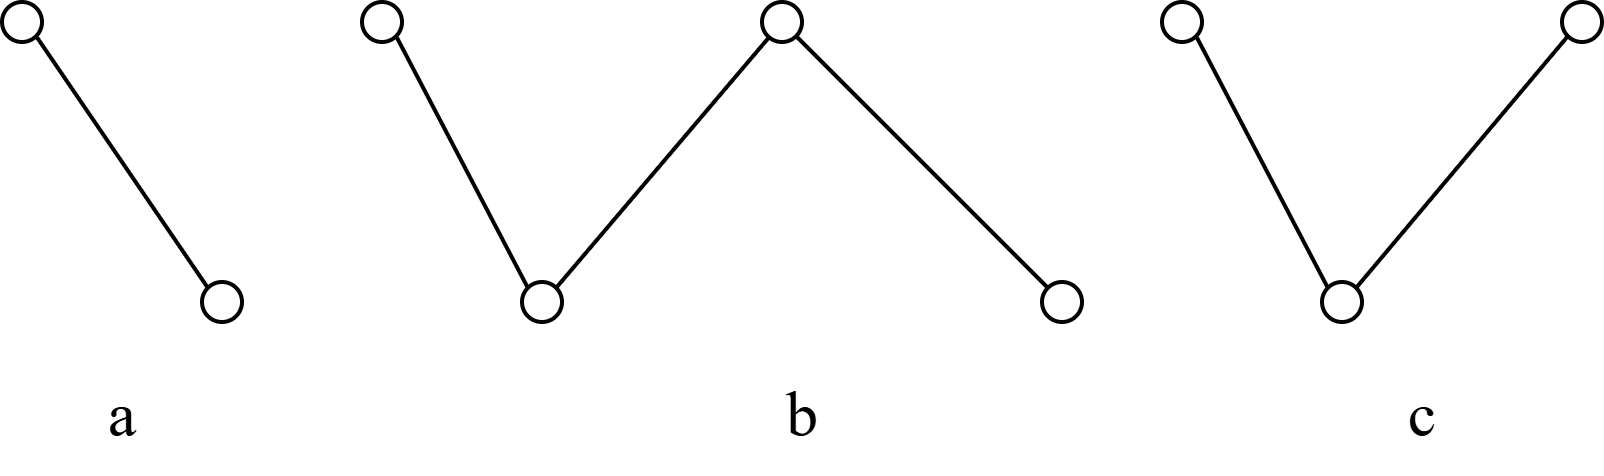
\includegraphics[width=0.8\textwidth]{images/1-1-1.png}
    \caption{Examples of Constrained Systems}
    \label{fig:1-1-1}
\end{figure}

\subsection{Degrees of Freedom}

\begin{definition}[Degrees of Freedom]
    The number of independent variables required to completely specify the configuration 
    of a system.
\end{definition}

In general, for a 3D object composed of $M$ moving parts, the number of degrees of 
freedom (DOF) is given by:

\begin{equation}
    \text{DOF} = 3M - N
\end{equation}

where $N$ is the number of independent constraints imposed on the system.

Let's consider the examples in Figure~\ref{fig:1-1-1}:

\begin{itemize}
    \item For case (a), two particles connected by a rod:
    \item 
        \begin{equation}
            \text{DOF} = 3 \times 2 - 1 = 5
        \end{equation}

        Here, the constraint is that the distance between the two particles is fixed.

    \item For case (b), four particles connected by rods where all angles are fixed:

        \begin{equation}
            \text{DOF} = 3 \times 4 - 3 \text{ (lengths)} - 3 \text{ (angles)} = 3 \text{ (COM)} + 3 \text{ (orientations)} = 6
        \end{equation}

        This is equivalent to describing the motion of a rigid body in 3D space, which 
        has 3 translational and 3 rotational degrees of freedom.

    \item For case (c), three particles connected by rods with one angle not fixed:

        \begin{equation}
            \text{DOF} = 3 \times 3 - 2 \text{ (lengths)} = 7
        \end{equation}
\end{itemize}

It's important to note that dynamical variables are not restricted to Cartesian 
coordinates. We can use any set of independent variables that uniquely specify the 
system's state, such as:

\begin{equation}
    \mathbf{r} = (x, y, z) = (r, \theta, \phi) = \dots
\end{equation}

\begin{figure}[ht]
    \centering
    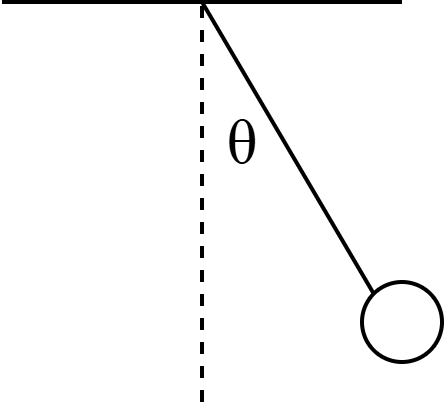
\includegraphics[width=0.3\textwidth]{images/1-1-2.png}
    \caption{Pendulum Example}
    \label{fig:1-1-2}
\end{figure}

Consider the simple pendulum shown in Figure~\ref{fig:1-1-2}. The system has only $1$ DOF.
We could choose $x$, $y$, or $\theta$ as the dynamical variable. 

We can introduce a set of generic degrees of freedom $q_i$, where $i = 1, 2, ..., N$, and 
$N$ is the number of degrees of freedom. For a constrained system, the position of any 
part of the system can be written as a function of these generalized coordinates:

\begin{equation}
    \mathbf{r}_\alpha = \mathbf{r}_\alpha(q_i, t), \quad \alpha = \text{index for particles}
\end{equation}

This form allows for the possibility of an explicit time dependence. If the position 
vectors can be expressed in this way, the system is said to be \textbf{holonomic}. 
Otherwise, it is  \textbf{nonholonomic}. Furthermore, if the relation between
 $\mathbf{r}_\alpha$ and $q_i$ is time-independent (i.e., 
 $\mathbf{r}_\alpha = \mathbf{r}_\alpha(q_i)$), the system is \textbf{scleronomic}; 
 otherwise, it is \textbf{rheonomic}.

\begin{figure}[ht]
    \centering
    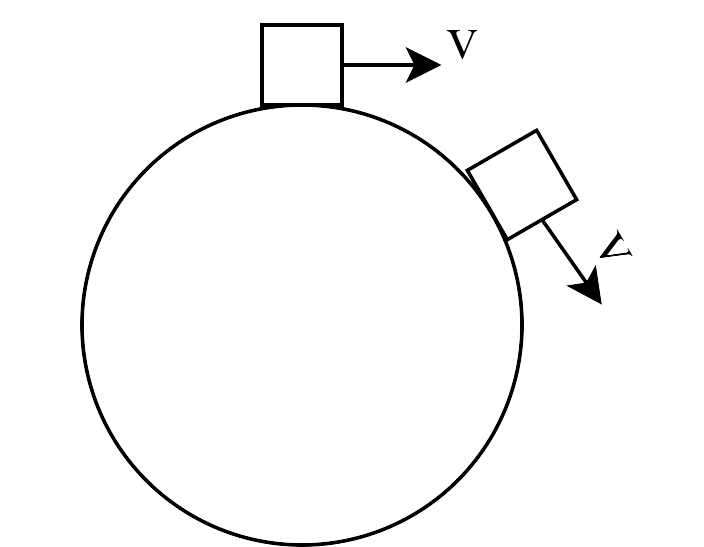
\includegraphics[width=0.3\textwidth]{images/1-1-3.png}
    \caption{Nonholonomic System Example}
    \label{fig:1-1-3}
\end{figure}

Nonholonomic systems are common.  In the example of the box on a surface in Figure 
\ref{fig:1-1-3}, the DOF increases from 2 to 3 when the box leaves the surface.

\subsection{Lagrangian Mechanics}

Consider a system described by the generalized coordinates $q_i$, where $i = 1, 2, ..., N$ 
(number of DOF). The positions of the system's parts can be written as 
$\mathbf{r}_\alpha = \mathbf{r}_\alpha(q_i, t)$. The fundamental problem is to determine 
the time evolution of these generalized coordinates, $q_i(t)$. These will satisfy a set 
of $N$ differential equations, known as the \textbf{equations of motion}.

Traditionally, Newton's laws of motion were used, which requires dealing with constraint 
forces:

\begin{enumerate}
    \item Determine the force $\mathbf{F}_\alpha$ acting on each part of the system at 
    position $\mathbf{r}_\alpha$.
    \item Apply Newton's second law, which gives a system of second-order ordinary 
    differential equations (ODEs):

    \begin{equation}
        \mathbf{F}_\alpha = m_\alpha \ddot{\mathbf{r}}_\alpha
    \end{equation}

    \item  Rewrite $\mathbf{r}_\alpha$ in terms of $q_i$. This can be challenging to 
    actually implement!
\end{enumerate}

Lagrangian mechanics provides an elegant way to avoid dealing with constraint forces 
directly.

Consider an infinitesimal change in position, $\delta \mathbf{r}_\alpha$. The work done 
by the force is:

\begin{equation}
    \delta W = \sum_{\alpha} \mathbf{F}_\alpha \cdot \delta \mathbf{r}_\alpha
\end{equation}

A crucial question arises: how much work is done if we change the generalized coordinates 
from $q_i$ to $q_i + \delta q_i$? Since $\mathbf{r}_\alpha = \mathbf{r}_\alpha(q_i, t)$, 
the variation in position can be written as:

\begin{equation}
    \delta \mathbf{r}_\alpha = \sum_{i} \frac{\partial \mathbf{r}_\alpha}{\partial q_i} \delta q_i
\end{equation}

This assumes that we only consider variations in the generalized coordinates, keeping 
$t$ constant. Thus:

\begin{align}
    \delta W &= \sum_{\alpha} \mathbf{F}_\alpha \cdot \left(\sum_{i} \frac{\partial \mathbf{r}_\alpha}{\partial q_i} \delta q_i \right) \\
             &= \sum_{i} \left(\sum_{\alpha} \mathbf{F}_{\alpha} \cdot \frac{ \partial \mathbf{r}_\alpha}{\partial q_i} \right) \delta q_i
\end{align}

We define the term in the parenthesis to be a \textbf{generalized force}:

\[
    F_i = \sum_{\alpha} \mathbf{F}_{\alpha} \cdot \frac{\partial \mathbf{r}_\alpha}{\partial q_i}
\]

Here, $F_i$ is the generalized force associated with the generalized coordinate $q_i$. It effectively represents the force component in the "allowed" direction defined by the variation in $q_i$.

Now let's consider the kinetic energy of a constrained system:

\begin{align}
    T &= \frac{1}{2} \sum_{\alpha} m_\alpha \dot{\mathbf{r}}_\alpha \cdot \dot{\mathbf{r}}_\alpha \\
      &= T(q_i, \dot{q_i}, t) \\
\end{align}

where,

\begin{align}
    \mathbf{r}_\alpha &= \mathbf{r}_\alpha(q_i, t) \\
    \dot{\mathbf{r}}_\alpha &= \sum_i \frac{\partial \mathbf{r}_\alpha}{\partial q_i} \dot{q_i} + \frac{\partial \mathbf{r}_\alpha}{\partial t}
\end{align}

Note that from the expression above, we have

\begin{equation}
    \frac{\partial \dot{\mathbf{r}}_\alpha}{\partial \dot{q_i}} = \frac{\partial \mathbf{r}_\alpha}{\partial q_i}
\end{equation}

We can compute the partial derivatives of the kinetic energy:

\begin{align}
    \frac {\partial T}{\partial q_i} &= \sum_\alpha m_\alpha \dot{\mathbf{r}}_\alpha \cdot \frac{\partial \dot{\mathbf{r}}_\alpha}{\partial q_i} \\
    \frac {\partial T}{\partial \dot{q_i}} &= \sum_\alpha m_\alpha \dot{\mathbf{r}}_\alpha \cdot \frac{\partial \dot{\mathbf{r}}_\alpha}{\partial \dot{q_i}} = \sum_\alpha m_\alpha \dot{\mathbf{r}}_\alpha \cdot \frac{\partial \mathbf{r}_\alpha}{\partial q_i}\\
\end{align}

Now, let's compute the time derivative of $\frac {\partial T}{\partial \dot{q_i}}$:

\begin{align}
    \frac{d}{dt} \left(\frac {\partial T}{\partial \dot{q_i}}\right) &= \sum_\alpha m_\alpha \left(\ddot{\mathbf{r}}_\alpha \cdot \frac{\partial \mathbf{r}_\alpha}{\partial q_i} + \dot{\mathbf{r}}_\alpha \cdot \frac{\partial \dot{\mathbf{r}}_\alpha}{\partial q_i}\right) \\
    &= \sum_\alpha \mathbf{F}_\alpha \cdot \frac{\partial \mathbf{r}_\alpha}{\partial q_i} + \frac{\partial T}{\partial q_i} \\
    &= F_i + \frac{\partial T}{\partial q_i} \\
\end{align}

Therefore, we have the following important relation:

\begin{equation}
    F_i = \frac{d}{dt} \left(\frac {\partial T}{\partial \dot{q_i}}\right) - \frac{\partial T}{\partial q_i}
\end{equation}

If we know the kinetic energy $T(q_i, \dot{q}_i, t)$, we can obtain the generalized force 
without directly calculating constraint forces! This provides a powerful generalization 
of $\mathbf{F} = m\mathbf{a}$ to a generic degree of freedom.